\section{Introduction}
\label{sec:intro}

Knowledge graph question answering (KGQA) aims to answer natural language questions by reasoning over large-scale structured Knowledge Graphs (KGs) \citep{jang2017kbqa}, where world knowledge is encoded as (subject, predicate, object) triples. Answering complex questions over KGs demands multi-hop reasoning, systematic path planning, and structural awareness of the underlying graph topology \citep{xiongenhancing}. The advent of Large Language Models (LLMs) \citep{brown2020language} has opened new opportunities for KGQA due to their strong language understanding and reasoning capabilities \citep{petroni2019language}.


\begin{figure}[h]
    \vspace{-10pt}
    \centering
    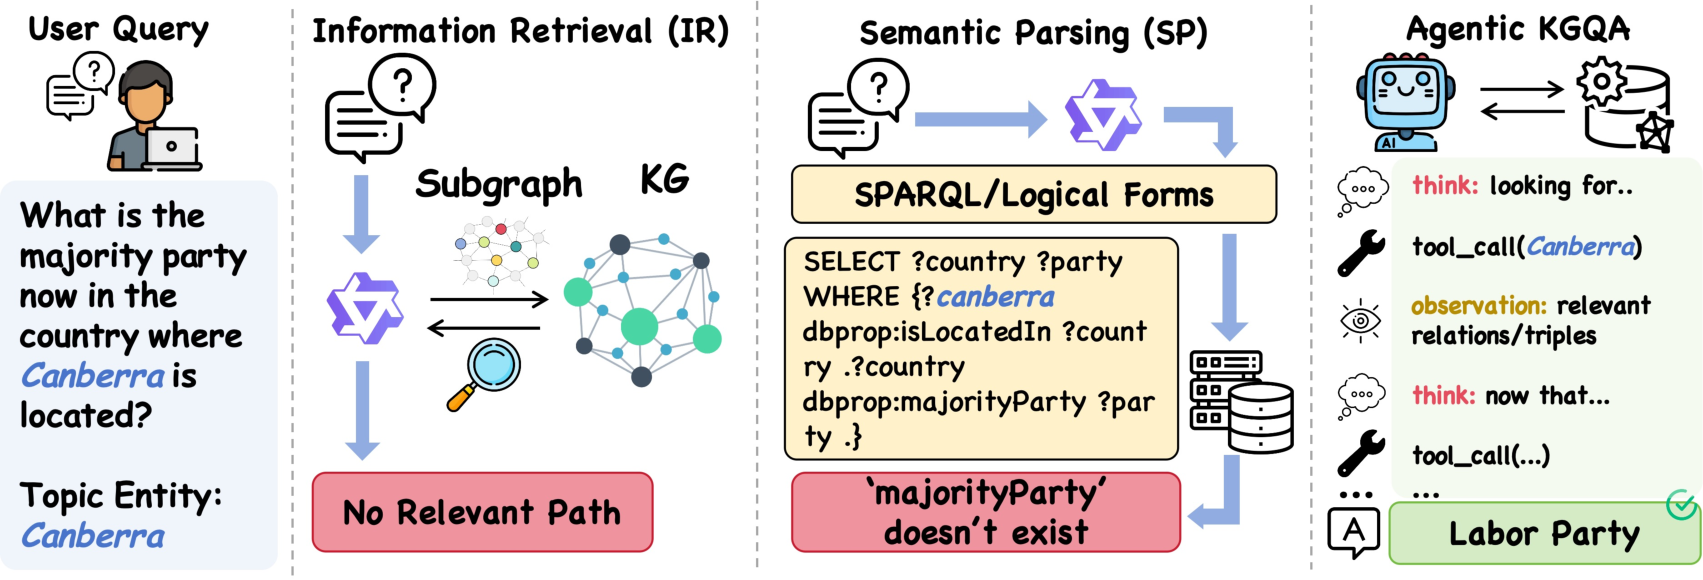
\includegraphics[width=\linewidth]{figures/figure1.pdf}
    \caption{Comparison of three KGQA paradigms.}
    \label{fig:paradigm-comparison}
    \vspace{-10pt}
\end{figure}


As illustrated in Figure~\ref{fig:paradigm-comparison}, traditional KGQA methods follow two main paradigms:
\textbf{Information Retrieval (IR) methods} \citep{Zhang_2022, dong2023bridgingkbtextgapleveraging, li2024chainofknowledgegroundinglargelanguage}, which retrieve relevant subgraphs and extract answers from the gathered evidence, and \textbf{Semantic Parsing (SP) methods} \citep{berant2013semantic, yih2015semantic, li2023fewshotincontextlearningknowledge, Luo_2024}, which translate questions into executable logical forms (e.g., SPARQL) to query KGs directly. 
However, both paradigms confine reasoning within a static, pre-defined scope, which severely limits their \textit{generalization to unseen reasoning structures} in real-world KGs \citep{auer2007dbpedia, bollacker2008freebase, vrandecic2014wikidata, xiong2025deliberate}.


% To overcome this limitation, recent \textbf{Agentic KGQA methods} empower LLMs to iteratively interact with the global KG via successive tool calls, dynamically refining their reasoning based on real-time KG feedback \citep{yao2023reactsynergizingreasoningacting, sun2023think}.
% Despite this progress, as shown in Table~\ref{tab:method-comparison}, existing approaches remain limited in several aspects. 
% \textbf{Prompting-based methods}~\citep{sun2023think,xu2024generate} offer flexible reasoning but lack the domain-specific adaptation needed to reliably navigate noisy and complex KGs.
% \textbf{Training-based methods}, on the other hand, lack unified capabilities: 
% RoG \citep{luo2023reasoning} restricts reasoning to predefined workflows, lacking \textit{autonomous interaction}; 
% KG-Agent \citep{jiang2025kg} relies on imitation without \textit{RL optimization} to break the demonstration ceiling; 
% existing RL methods (e.g., KG-R1 \citep{song2025efficient}) often rely on pre-sampled subgraphs rather than the \textit{global KG}.
% Critically, recent studies have consistently shown that RL optimization requires a competent SFT prior: without sufficient exploration capacity, the agent cannot discover rewarding trajectories, rendering policy optimization ineffective \citep{Guo_2025, zhang2026asteragenticscalingtoolintegrated, xiong2026scaling}.
% This raises a central question: \textit{How can an agent build a robust exploration foundation on KGs to push the boundaries of its reasoning capacity?}


To overcome this limitation, recent \textbf{Agentic KGQA methods} allow LLMs to interact with KGs via successive tool calls, dynamically refining their reasoning based on real-time feedback \citep{yao2023reactsynergizingreasoningacting, sun2023think}.
However, as shown in Table~\ref{tab:method-comparison}, existing approaches still exhibit notable limitations.
Prompting-based and SFT-based methods \citep{sun2023think,xu2024generate,luo2023reasoning,jiang2025kg} often hit performance ceilings due to \textit{insufficient environmental adaptation}. 
Meanwhile, existing RL-based methods \citep{song2025efficient} suffer from a critical exploration bottleneck: they apply policy optimization on pre-extracted subgraphs without a comprehensive SFT prior. 
By confining their training to simplified environments, they severely restrict the agent's search space, hindering effective navigation of the vast, noisy \textit{global KG} during inference.
Most importantly, recent studies \citep{Guo_2025, zhang2026asteragenticscalingtoolintegrated, xiong2026scaling} consistently demonstrate that RL requires a structurally diverse SFT foundation; without a broad exploration prior, policy optimization on global KGs proves ineffective.
This raises a central question: \textit{How can an agent build a robust exploration foundation to push the boundaries of its reasoning capacity?}


\begin{table}[t]
  \caption{Comparison of GraphWalker with existing agentic KGQA methods across three key properties: \textbf{\textit{Global KG}} (operating on global KGs rather than pre-extracted subgraphs), \textbf{\textit{Autonomous Interaction}} (interacting autonomously rather than via pre-defined workflows), and \textbf{\textit{RL Optimization}} (incorporating reinforcement learning to optimize reasoning policies).}
  \vspace{-6pt}
  \label{tab:method-comparison}
  \centering
  \small
  \setlength{\tabcolsep}{5pt}
  \renewcommand{\arraystretch}{1.25}
  \begin{tabular}{l|l|ccc}
  \toprule
  \textbf{Type}
  & \textbf{Method}
  & \textbf{\shortstack{Global\\KG}}
  & \textbf{\shortstack{Autonomous\\Interaction}}
  & \textbf{\shortstack{RL \\ Optimization}} \\
  \midrule
  \multirow{2}{*}{Prompting}
  & ToG \citep{sun2023think}         & \cmark & \cmark & \xmark \\
  & GoG \citep{xu2024generate}       & \cmark & \cmark & \xmark \\
  \midrule
  \multirow{4}{*}{Training}
  & RoG \citep{luo2023reasoning}     & \xmark & \xmark & \xmark \\
  & KBQA-o1 \citep{luo2025kbqa}     & \cmark & \cmark & \xmark \\
  & KG-Agent \citep{jiang2025kg}    & \cmark & \cmark & \xmark \\
  & KG-R1 \citep{song2025efficient} & \xmark & \cmark & \cmark \\
  \midrule
  \rowcolor{blue!8}
  \multirow{1}{*}{\textbf{Ours}}
  & \textbf{GraphWalker}             & \cmark & \cmark & \cmark \\
  \bottomrule
  \end{tabular}
  \vspace{-14pt}
\end{table}


To address these issues, this paper proposes \textit{GraphWalker}, a framework that autonomously synthesizes interaction trajectories for \textit{Stage-Wise Fine-tuning}, followed by lightweight RL with a sparse exact-match (EM) reward.
Specifically, the two SFT stages directly target the aforementioned exploration and robustness bottlenecks. 
First, we conduct \textit{Constrained Random Walk (CRW)} on the KG and synthesize \textit{GraphSynth}, a corpus of 15k diverse trajectories that establishes a broad exploration prior.
Second, we construct \textit{GraphRoll}, a dataset of 6k distilled expert trajectories that equips the agent with reflection and error recovery capabilities.
Importantly, we demonstrate that the first stage serves as a
\textit{mid-training exploration scaffold}, which unlocks a higher performance ceiling during subsequent RL.

% To address these issues, this paper proposes \textit{GraphWalker}, a framework that autonomously synthesizes interaction trajectories for a \textit{Stage-Wise Fine-tuning}, followed by lightweight RL with a sparse exact-match reward.
% Specifically, the two SFT stages directly target the aforementioned exploration and robustness bottlenecks.
% First, to overcome the restricted search space caused by bypassing broad pre-training, a \textit{Constrained Random Walk (CRW)} synthesizes \textit{GraphSynth}---a corpus of 15k structurally diverse trajectories that establishes a broad exploration prior directly on the global KG.
% Second, to ensure robust navigation in massive, noisy environments, \textit{GraphRoll} provides 6k distilled expert trajectories that equip the agent with essential reflection and error recovery capabilities.
% Importantly, this paper demonstrates that the stage-wise SFT successfully builds the missing exploration foundation, unlocking a significantly higher performance ceiling for the final RL stage.

Our main contributions are summarized as follows:

\begin{itemize}[leftmargin=*]
    \vspace{-6pt}
    \item We identify the lack of an exploration prior as the core bottleneck in agentic KGQA generalization, and propose GraphWalker to address this limitation through two complementary datasets: \textit{GraphSynth}, 15k autonomously constructed, structurally diverse interaction trajectories, and \textit{GraphRoll}, 6k curated high-quality expert trajectories.
    
    \item We introduce a \textit{Stage-Wise SFT curriculum} to build a robust exploration foundation. By sequentially establishing a broad search prior and instilling error recovery, our method enables the agent to navigate vast, noisy KGs, unlocking a higher performance ceiling for subsequent RL optimization.
    
    \item Extensive experiments demonstrate that GraphWalker achieves SOTA performance on WebQSP and CWQ. Strong zero-shot results on GrailQA and our GraphWalkerBench confirm its superior robustness and generalization to unseen reasoning structures.
\end{itemize}
